\documentclass[10pt,journal,a4paper]{IEEEtran}
\usepackage{graphicx,booktabs,amsmath,amssymb,array,cite,url,xcolor,balance}
\usepackage[hidelinks]{hyperref}
\graphicspath{{../results/cost_stable_confirmatory/final_analysis/}}
\title{
\includegraphics[width=\textwidth]{baic2026_header.png}\\[-0.35em]
CostStableEHOA: Budget-Feasible and Stability-Aware Feature Selection Using Resampled Lower-Confidence Utility}
\author{Amirreza Ghaffarian\\Graduate Student, Islamic Azad University}
\begin{document}
\maketitle
\begin{abstract}
Wrapper feature selection can produce accurate but costly and unstable subsets. This paper presents CostStableEHOA, a constrained extension of the Enhanced Hiking Optimization Algorithm (EHOA). Candidate masks that violate a hard acquisition budget are repaired by removing the active feature with the smallest stability-adjusted utility-to-cost ratio. Utility is the lower confidence bound (LCB) of mutual information estimated over training-only bootstrap resamples; the original EHOA fitness is unchanged. A confirmatory nested evaluation compared EHOA with random, cheapest-first, mutual-information, and stable-LCB repairs on ten public classification data sets. The experiment retained 300 complete runs and 300 masks, with no duplicate keys, missing values, failed runs, or budget violations. Across data-set aggregates, stable-LCB reduced selected-cost ratio from 0.4782 to 0.2775 and increased Nogueira stability from 0.1229 to 0.2554 relative to EHOA. Two-sided Wilcoxon tests remained significant after within-metric Holm correction ($p=0.0078$ for cost and $p=0.0156$ for stability). Balanced accuracy changed from 0.8301 to 0.8280 and was not significant ($p=1.0$ after correction). Stable-LCB was not significantly superior to simpler budget repairs. The evidence therefore supports a cost--stability trade-off, not universal predictive superiority.
\end{abstract}
\begin{IEEEkeywords}feature selection, acquisition cost, stability, mutual information, lower confidence bound, EHOA, nested validation\end{IEEEkeywords}

\section{Introduction}
Feature selection reduces dimensionality, measurement burden, and model complexity. Wrapper methods directly optimize downstream predictive behavior but can be computationally expensive and sensitive to small changes in the training sample. This sensitivity is important whenever selected variables are interpreted or repeatedly acquired. Nogueira \emph{et al.} formalized a chance-corrected stability measure suitable for selectors returning subsets of varying size \cite{nogueira2018}.

EHOA combines chaotic initialization, dynamic sweep control, velocity-inspired movement, and binary transfer for medical feature selection \cite{hegazy2026}. Its objective balances cross-validated error and subset size, but it does not impose a hard feature-acquisition budget or explicitly prefer evidence that is reproducible under resampling. Cost-constrained feature selection has been studied independently \cite{jagdhuber2020}; therefore neither cost nor repair is claimed as novel in isolation.

This work makes three scoped contributions: (1) a hard-budget repair integrated into every EHOA candidate evaluation; (2) a stability-adjusted utility defined as a resampled mutual-information LCB divided by feature cost; and (3) a paired confirmatory comparison against three simpler repairs under a common budget and unchanged wrapper fitness. The claim is incremental and mechanism-specific.

\section{Related Work}
Metaheuristic feature selection searches a combinatorial mask space while using a predictive model as a subset evaluator. Recent methods employ multiple strategies, adaptive control, and relevance guidance; these are established concepts rather than isolated novelties.

Cost-sensitive selection introduces nonuniform acquisition costs, often through constrained optimization or a penalty term \cite{jagdhuber2020}. A penalty, however, may still return an infeasible mask and requires tuning a trade-off coefficient. A repair operator enforces feasibility exactly. The present method differs from cheapest-first or single-sample relevance repair by discounting relevance estimates that vary across resamples.

Feature-selection stability is distinct from accuracy. Nogueira's estimator corrects overlap for chance and accommodates different subset cardinalities \cite{nogueira2018}. We use it only as an external outcome; it is not inserted into EHOA's fitness, avoiding a change to the baseline objective.

\section{Method}
Let $\mathbf z\in\{0,1\}^D$ be a mask, $c_j>0$ the acquisition cost of feature $j$, and $B$ the hard budget. Feasibility requires
\begin{equation}\sum_{j=1}^{D}z_jc_j\le B.\end{equation}
For bootstrap resample $b=1,\ldots,R$, mutual information $I_{jb}$ is estimated using only the outer-training partition. Stable utility and utility-to-cost ratio are
\begin{equation}
u_j=\max\!\left(0,\bar I_j-z_{\alpha}s_j\right),\qquad q_j=\frac{u_j}{\max(c_j,\epsilon)}.
\end{equation}
Here $s_j$ is the across-resample standard deviation and $z_{\alpha}$ controls conservatism. When a candidate is infeasible, the active feature with minimum $q_j$ is removed repeatedly. If repair empties the mask, the feasible feature with maximum $q_j$ is restored.

\begin{figure}[t]
\small\hrule\vspace{3pt}
\textbf{Stable-LCB repair}\par
\emph{Input:} mask $\mathbf z$, costs $\mathbf c$, budget $B$, utility $\mathbf u$\par
\textbf{while} $\mathbf c^T\mathbf z>B$ \textbf{do}\par
\quad $j\leftarrow\arg\min_{k:z_k=1}u_k/(c_k+\epsilon)$; $z_j\leftarrow0$\par
\textbf{if} $\|\mathbf z\|_0=0$ \textbf{then} restore the feasible feature with largest ratio\par
\emph{Return:} feasible $\mathbf z$
\vspace{3pt}\hrule
\caption{Hard-budget repair used before each candidate evaluation.}
\end{figure}

The inherited EHOA population update, binary transfer, and fitness are not modified. This isolates the effect of repair. Four constrained variants use identical search settings but rank removals randomly, by cost, by mutual information, or by stable-LCB.

\section{Experimental Protocol}
Ten public data sets were used: Breast Cancer, Wine, Ionosphere, Sonar, Dermatology, Spambase, Parkinsons, Hill-Valley, Steel Plates Fault, and Madelon. Each method used two fixed seeds and three stratified outer folds, yielding $10\times5\times2\times3=300$ runs. Inner three-fold validation was used by the wrapper. Population size was 8, iterations were 10, and the EHOA accuracy weight was 0.99.

Feature costs were generated once per data set from a deterministic log-normal model independent of labels. The budget was 30\% of total cost. This design tests controlled cost sensitivity, not domain-specific monetary costs. Preprocessing, utility estimation, search, and model fitting used outer-training data only. The outer test fold was used once for evaluation. K-nearest neighbors was the primary classifier.

For inference, six runs were first averaged within each data set and method. The ten data sets, not the 300 rows, were treated as independent units. Friedman tests assessed overall differences. Stable-LCB was compared with four controls using two-sided paired Wilcoxon tests; four comparisons within each metric were Holm-corrected \cite{demsar2006}.

\section{Results}
The audit found 300 expected rows, 300 masks, zero missing values, zero duplicate experiment keys, and zero budget violations. Table~\ref{tab:overall} reports data-set-level means.

\begin{table}[t]
\caption{Mean results across ten data sets. Higher is better for balanced accuracy and stability; lower is better for cost and size.}
\label{tab:overall}\centering\scriptsize
\resizebox{\columnwidth}{!}{%
\begin{tabular}{lrrrrr}\toprule
Method & Balanced accuracy & Cost ratio & Selected features & Nogueira stability & Runtime (s)\\\midrule
EHOA & 0.8301 & 0.4782 & 42.07 & 0.1229 & 1.785\\
Budget-random & 0.8288 & 0.2724 & 31.87 & 0.1403 & 1.653\\
Budget-cheapest & 0.8324 & 0.2728 & 35.18 & 0.2552 & 1.694\\
Budget-MI & \textbf{0.8331} & 0.2735 & \textbf{27.95} & 0.2335 & 1.622\\
Budget-stable-LCB & 0.8280 & 0.2775 & 30.98 & \textbf{0.2554} & \textbf{1.613}\\\bottomrule
\end{tabular}}
\end{table}

Relative to EHOA, stable-LCB lowered cost ratio by 0.2007 on average and did so on all ten data sets. The paired $p$-value was 0.00195 and Holm-adjusted $p=0.00781$. Stability increased by 0.1325, with nine wins and one loss; raw $p=0.00391$ and adjusted $p=0.01563$. Balanced-accuracy difference was $-0.00209$, with six numerical wins and four losses; raw $p=0.5566$ and adjusted $p=1.0$. A data-set bootstrap 95\% interval for the accuracy difference was approximately $[-0.0177,0.0087]$, so formal non-inferiority under a small margin is not established.

\begin{figure}[t]\centering
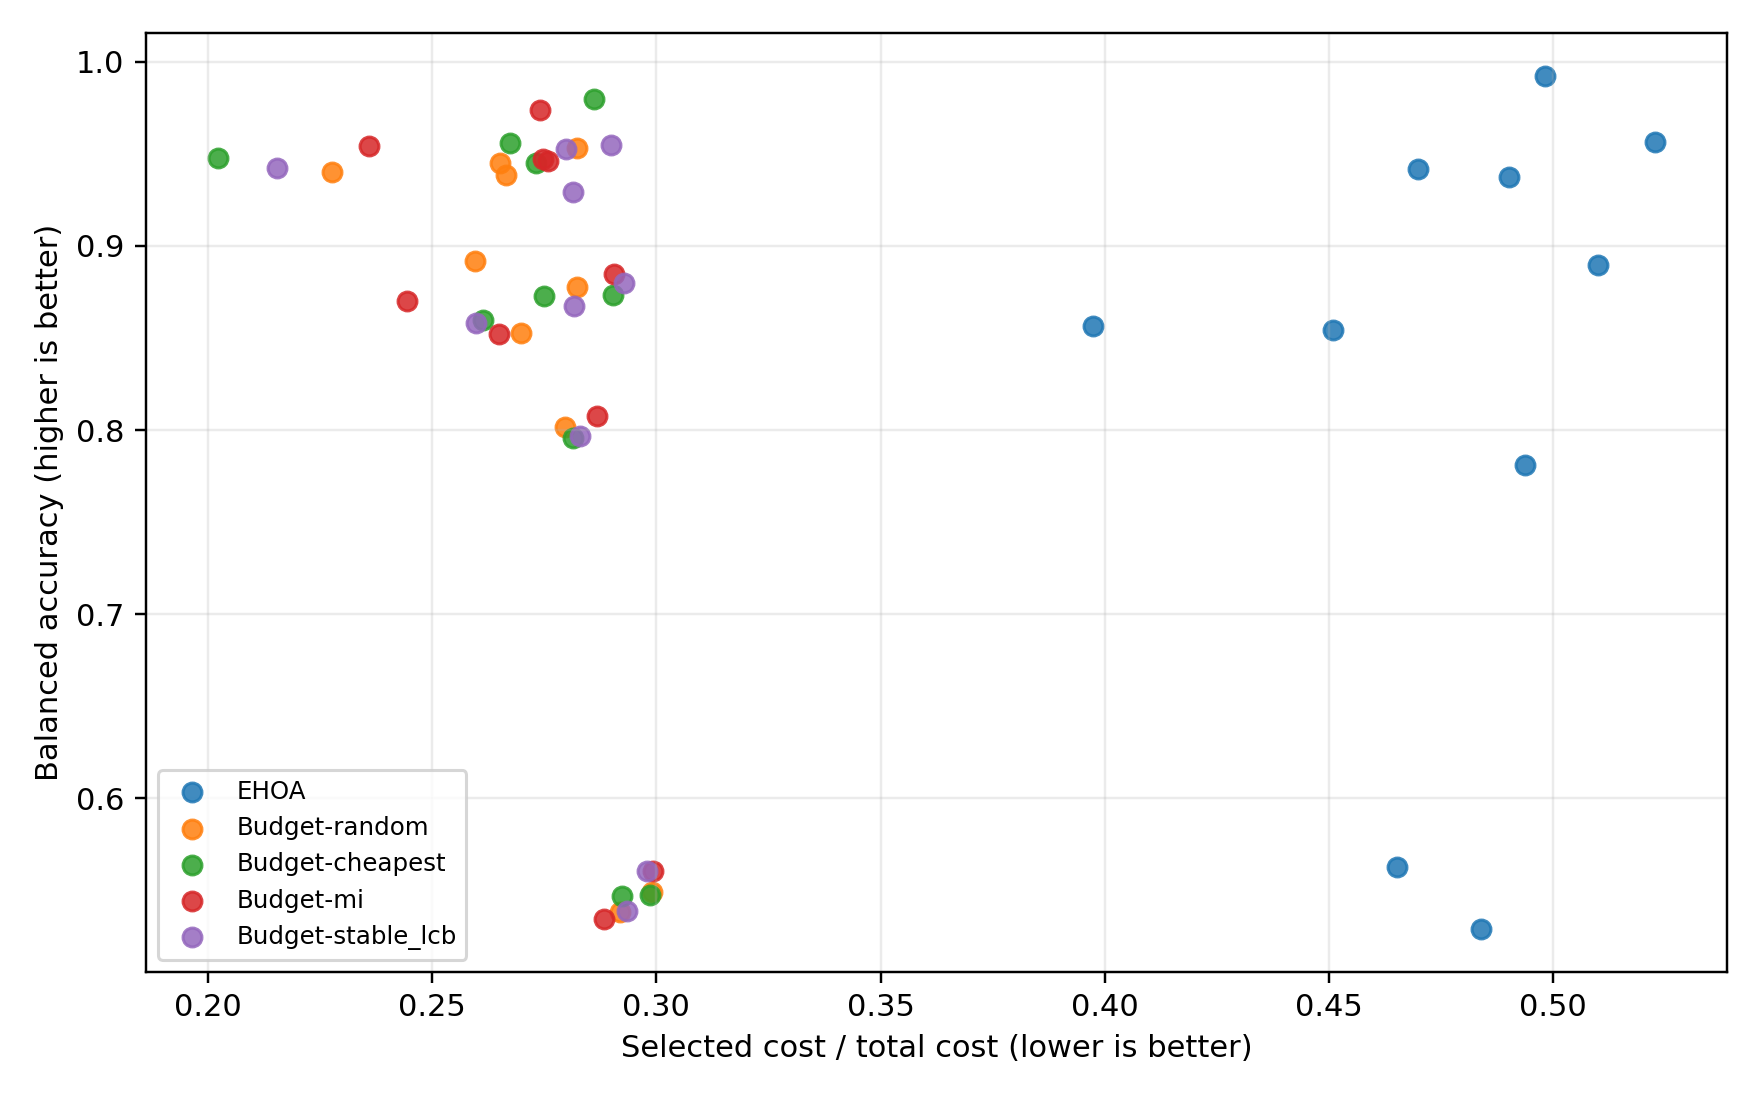
\includegraphics[width=\columnwidth]{accuracy_cost_tradeoff.png}
\caption{Accuracy--cost outcomes. The preferred direction is upper left.}
\label{fig:tradeoff}
\end{figure}

Against Budget-MI, stable-LCB had mean accuracy difference $-0.00509$ and stability difference $+0.02190$; neither was significant after correction. Its stability was nearly identical to cheapest-first repair. Thus the budget constraint explains the clear cost reduction, while the LCB ranking does not demonstrate universal superiority over simpler feasible repairs.

\section{Discussion}
The strongest evidence concerns two objectives neglected by unconstrained EHOA. Stable-LCB used approximately 42\% less selected cost relative to EHOA, computed as $(0.4782-0.2775)/0.4782$, and more than doubled chance-corrected stability. Predictive performance remained close on average, but absence of significance is not proof of equivalence.

The results also expose an important boundary. Budget-MI achieved the highest mean balanced accuracy and the lowest mean subset size. Stable-LCB's highest average stability did not translate into a significant advantage over all budget controls. Consequently, ``best algorithm,'' ``universal accuracy improvement,'' and ``first cost-aware selector'' would be unsupported claims. A defensible contribution is the exact LCB-per-cost repair within EHOA and its audited cost--stability behavior.

\section{Threats to Validity}
Synthetic costs may not reflect correlated, grouped, or time-varying costs in a real application. Ten data sets provide limited power for cross-data-set inference. Only two seeds, three outer folds, one primary classifier, and a modest search budget were used. Mutual information can underestimate multivariate interactions. Finally, the study evaluates one cost budget; conclusions may change under tighter or looser constraints.

\section{Detailed Results and Reproducibility}
Table~\ref{tab:detail-en} reports the balanced-accuracy difference between stable-LCB and EHOA together with the two main outcomes for each data set. The larger loss on Steel Plates Fault is the principal reason for the negative overall mean accuracy difference, whereas six data sets show a positive numerical difference. This heterogeneity motivates data-set-level reporting and rules out a universal-superiority claim.

\begin{table}[t]
\caption{Data-set-level stable-LCB results. $\Delta BA$ is relative to EHOA.}
\label{tab:detail-en}\centering\scriptsize
\begin{tabular}{lrrr}\toprule
Data set & $\Delta BA$ & Cost ratio & Stability\\\midrule
Breast Cancer & -0.0038 & 0.280 & 0.206\\
Dermatology & +0.0171 & 0.290 & 0.355\\
Hill Valley & +0.0099 & 0.294 & 0.110\\
Ionosphere & +0.0108 & 0.282 & 0.304\\
Madelon & -0.0021 & 0.298 & 0.181\\
Parkinsons & +0.0037 & 0.260 & 0.186\\
Sonar & +0.0155 & 0.283 & 0.054\\
Spambase & -0.0098 & 0.293 & 0.475\\
Steel Plates Fault & -0.0632 & 0.281 & 0.328\\
Wine & +0.0009 & 0.215 & 0.354\\\bottomrule
\end{tabular}
\end{table}

All 300 raw rows, 300 binary masks, random seeds, configuration hash, analysis code, and automated tests are retained. A clean execution of the delivered package passes 28 tests and regenerates the reported statistical tables. These artifacts permit independent auditing of the claims and distinguish confirmatory outputs from rejected exploratory candidates.

\begin{figure}[t]\centering
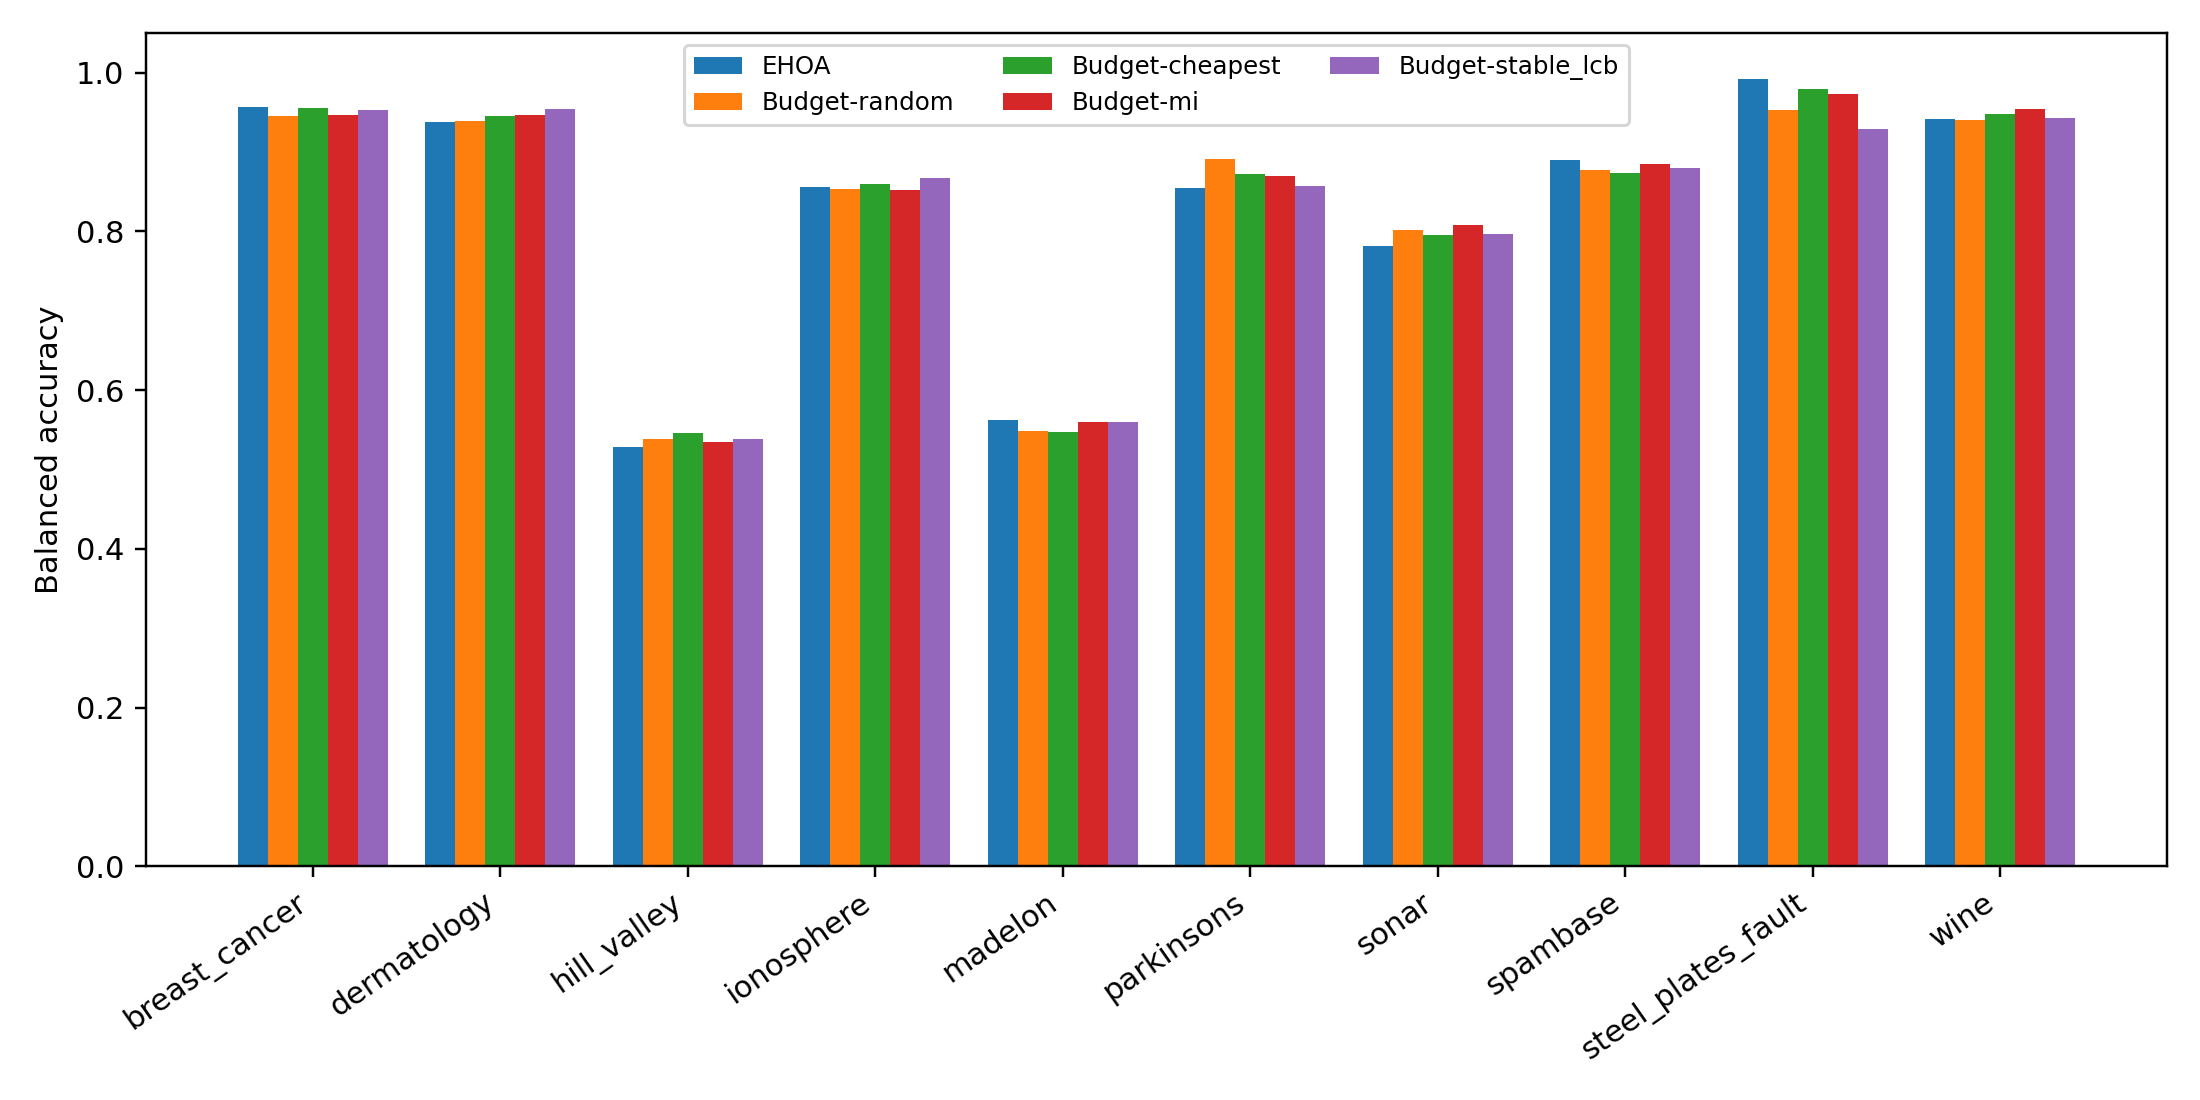
\includegraphics[width=\columnwidth]{balanced_accuracy_by_dataset.png}
\caption{Balanced accuracy of the five methods on each data set. Method rankings are not uniform across data sets.}
\label{fig:ba-detail}
\end{figure}

\balance\section{Conclusion}
CostStableEHOA enforced a hard acquisition budget in every run and significantly improved selected cost and subset stability relative to EHOA, without a statistically detectable balanced-accuracy change. It did not significantly dominate simpler budget repairs. The method should therefore be viewed as an incremental, reproducible cost--stability mechanism rather than a universally superior predictor. Code, configuration, all 300 run rows, masks, statistical outputs, and figures accompany the report.

\begin{thebibliography}{00}
\bibitem{hegazy2026} A. E. Hegazy, M. A. Makhlouf, O. A. M. Salem, and B. Hafiz, ``An enhanced Hiking optimization algorithm for accurate and interpretable feature selection in medical data classification,'' \emph{Cluster Computing}, vol. 29, p. 244, 2026, doi: 10.1007/s10586-026-05946-9.
\bibitem{nogueira2018} S. Nogueira, K. Sechidis, and G. Brown, ``On the stability of feature selection algorithms,'' \emph{J. Mach. Learn. Res.}, vol. 18, no. 174, pp. 1--54, 2018.
\bibitem{jagdhuber2020} R. Jagdhuber \emph{et al.}, ``Cost-constrained feature selection in binary classification,'' \emph{Computational Statistics}, vol. 35, pp. 1419--1440, 2020.
\bibitem{demsar2006} J. Demsar, ``Statistical comparisons of classifiers over multiple data sets,'' \emph{J. Mach. Learn. Res.}, vol. 7, pp. 1--30, 2006.
\end{thebibliography}
\end{document}
